\paragraph*{The relationship between network size and nestedness}\mbox{}\\
Disentangling species richness (the sum of host and parasite richness) from nestedness is difficult, and many nestedness measures scale with species richness (Figure \ref{fig:richnessEffect}). Comparisons of properties across networks of different sizes is a non-trivial problem, and one potential solution is the implementation of a null modeling approach. In our case, we repeatedly shuffled links between hosts and helminths in each network, while maintaining both parasite host range (i.e., the number of host species a given parasite infects), and parasite species richness (i.e., the number of parasite species a host is infected by). For each network, we produced 1000 randomized networks, creating a distribution of spectral radii. Using these null distributions, we calculated $z$-scores, which measure the degree of divergence of the empirical network from the randomized null networks. Below, we present the correlations between alternative measures of network nestedness ($\eta$ \parencite{jonhson2013factors}, spectral radius, NODF, and $NODF_c$) as well as z-transformed versions of NODF and spectral radius. Nestedness as measured by $\eta$ was not standardized, as null model randomization for this measure is difficult, as randomized networks maintaining aspects of the degree distribution of host and parasite species will result in the same $\eta$ value as the empirical network. 


\begin{figure}[H]
  \begin{center}
      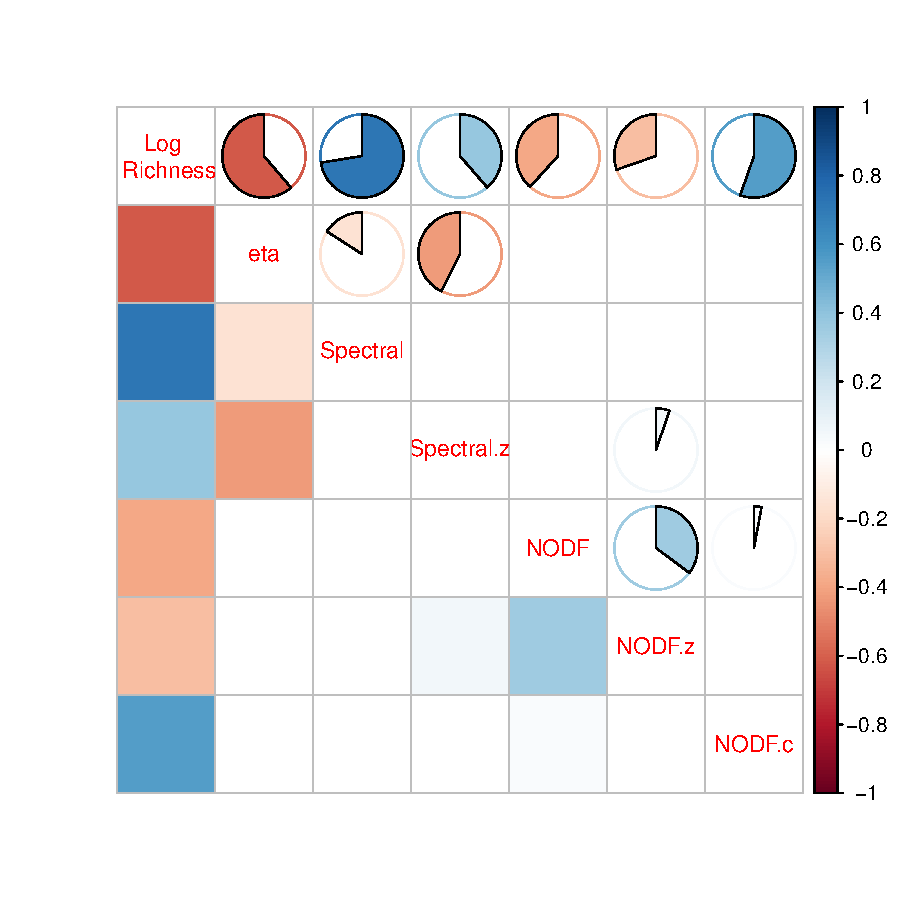
\includegraphics[width=\textwidth]{HelmBiogeog/Figures/Netsize_corplot.pdf}
    \caption[Relationship between network size and alternative measures of nestedness]{Correlogram visualizing Pearson's correlation coefficients between network size (log species richness) and alternative measures of network nestedness in our data. Shaded squares represent significant correlations (p-value $<0.05$). All measures of nestedness ($\eta$ \parencite{jonhson2013factors}, spectral radius, and NODF, as well as z-scores of the latter two based on null randomizations) are significantly correlated with network size in our dataset}
    \label{fig:richnessEffect}
  \end{center}
\end{figure}


\begin{figure}[H]
  \begin{center}
    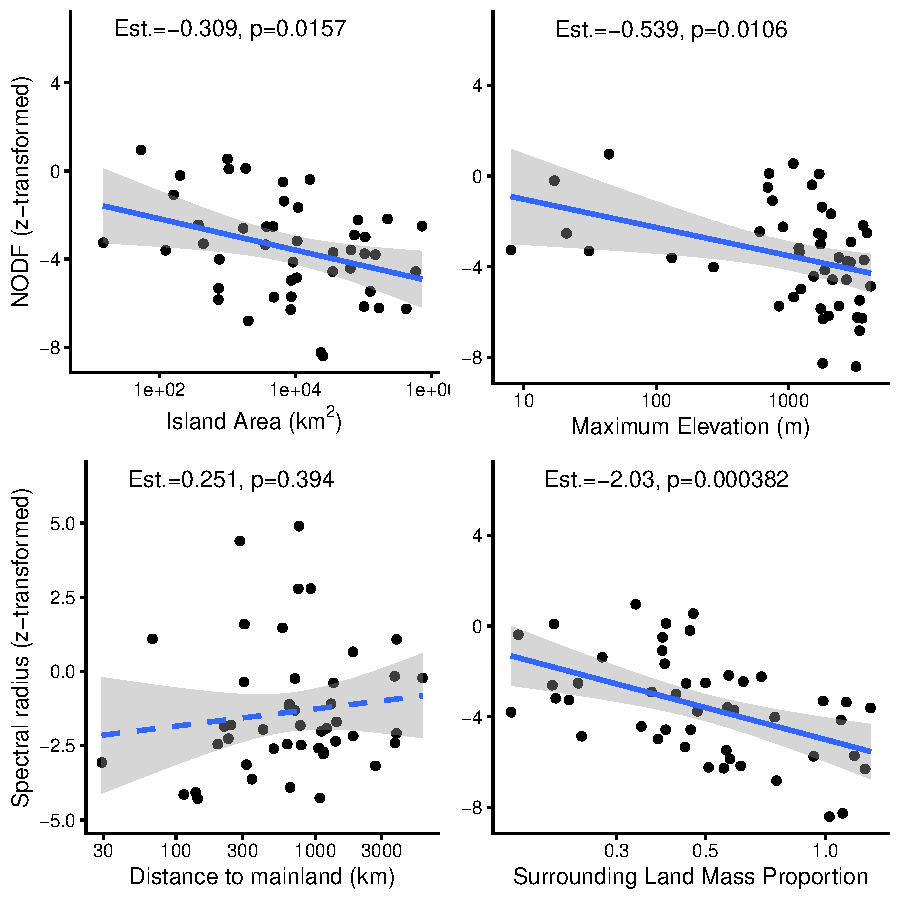
\includegraphics[width=\textwidth]{HelmBiogeog/Figures/NODF.z_Plots_Supplement.pdf}
    \caption[Relationship between NODF and island characteristics]{Recreation of Figure \ref{fig:networkBG} of the main text using z-transformed NODF as our nestedness metric of comparison. Despite null modeling approaches, this metric may still be sensitive to network size, and this gives conflicting results to those observed in $NODF_c$. }
    \label{fig:NODF.z_Results}
  \end{center}
\end{figure}

\clearpage

\begin{figure}[H]
  \begin{center}
    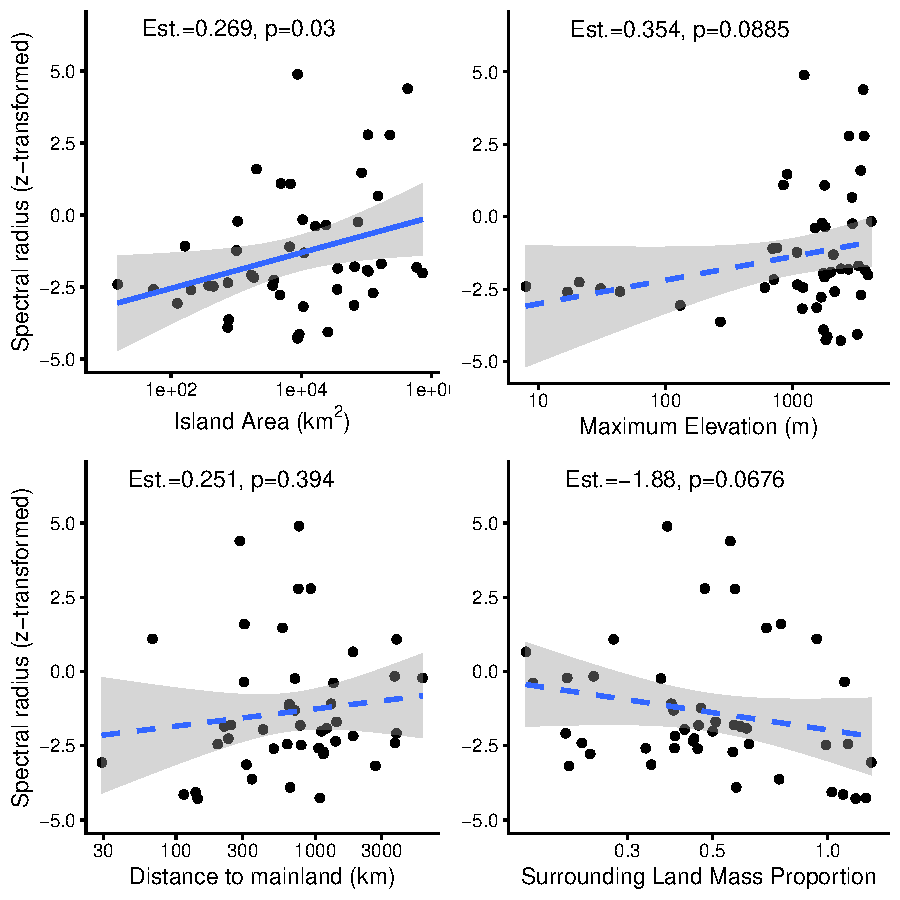
\includegraphics[width=\textwidth]{HelmBiogeog/Figures/Spectral.z_Plots_Supplement.pdf}
    \caption[Relationship between spectral radius and island characteristics]{Recreation of Figure \ref{fig:networkBG} of the main text using z-transformed spectral radius as our nestedness metric of comparison. In contrast to z-standardized NODF, spectral radius yields qualitatively similiar results to $NODF_c$ after z-transformation.}
    \label{fig:Spectral.z_Results}
  \end{center}
\end{figure}

\paragraph*{Statistical Analysis}\mbox{}\\
In the main text, we used a negative binomial modeling multivariate regression approach to model the effects of island characteristics on species diversity. This approach greatly minimizes residual deviance compared to both Poisson and Quasi-Poisson GLMs \ref{tab:host_div_deviance}. Models incorporating island area and isolation as measured by SLMP yielded lowest AIC values, and as such are presented in the main text. 

\begin{table}[ht]
\centering
\caption[Model deviance diagnostics for host diversity models]{Model deviance diagnostics for host diversity models.}
\label{tab:host_div_deviance}
\resizebox{\textwidth}{!}{%
\begin{tabular}{lrrrr}
\hline
Model & Residual deviance & Residual df & AIC & Deviance/df \\
\hline
Poisson: Area + SLMP & 5621.91 & 55 & 5873.20 & 102.22 \\
Quasi-Poisson: Area + SLMP & 3497.06 & 55 & -- & 63.58 \\
Negative binomial: Area + Distance & 65.10 & 55 & 488.86 & 1.18 \\
Negative binomial: Area + SLMP & 63.90 & 55 & 481.30 & 1.16 \\
Negative binomial: Elevation + Distance & 69.24 & 55 & 515.87 & 1.26 \\
Negative binomial: Elevation + SLMP & 68.08 & 55 & 509.48 & 1.24 \\
\hline
\end{tabular}%
}
\end{table}


Below, we report model diagnostic plots for the three models in the main text which show significant relationships between island characteristics and network properties. 

\begin{figure}[H]
  \begin{center}
    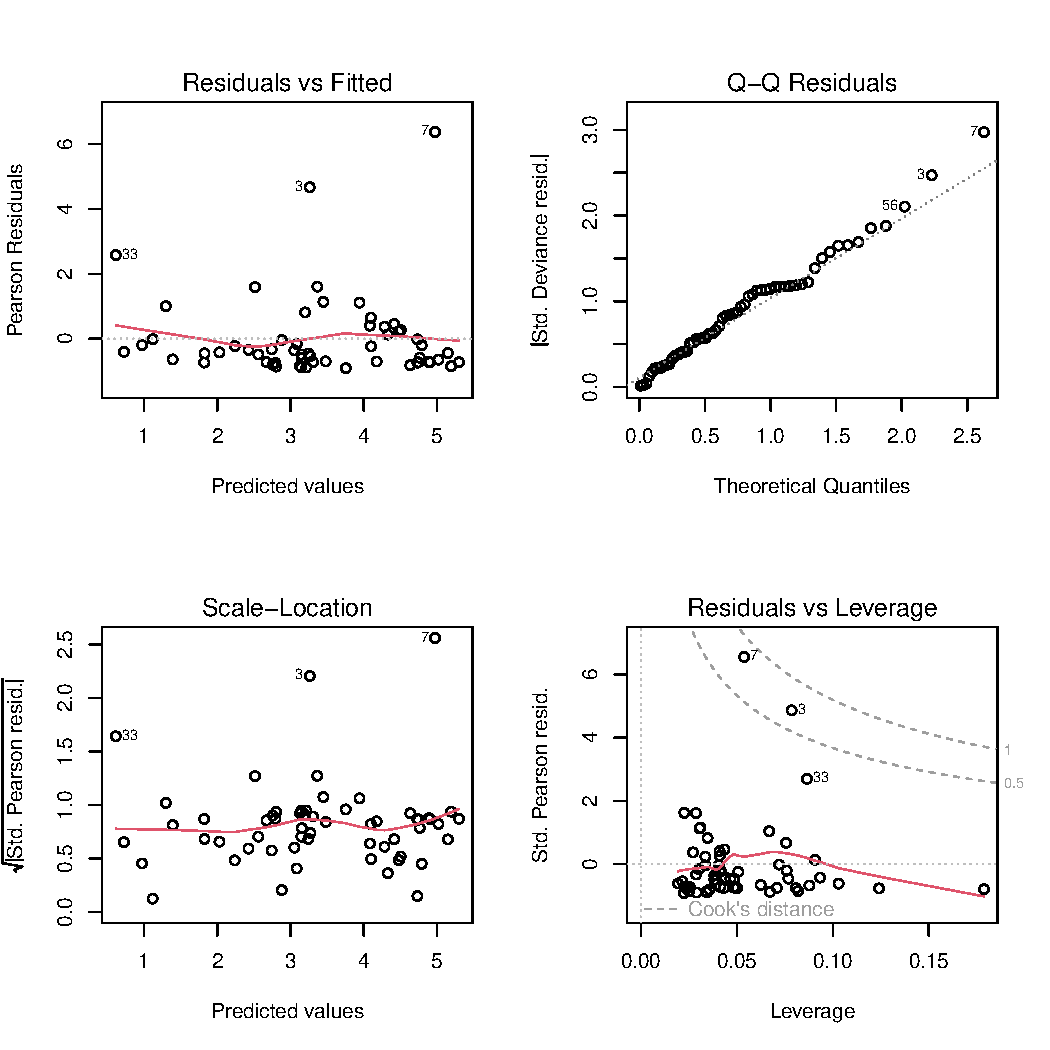
\includegraphics[width=\textwidth]{HelmBiogeog/Figures/ParDiv_diagnostics.pdf}
    \caption[Parasite richness model diagnostics]{Model diagnostics plots for our negative binomial model of \textbf{parasite richness} across islands, including residual vs fitted values (top left), Q-Q plot (top right), scale-location (bottom left), and residual vs leverage plot (bottom right), with dotted lines representing Cook's distance contours of 0.5 and 1, respectively. }
    \label{fig:parDivdiagnostics}
  \end{center}
\end{figure}

\begin{figure}[H]
  \begin{center}
    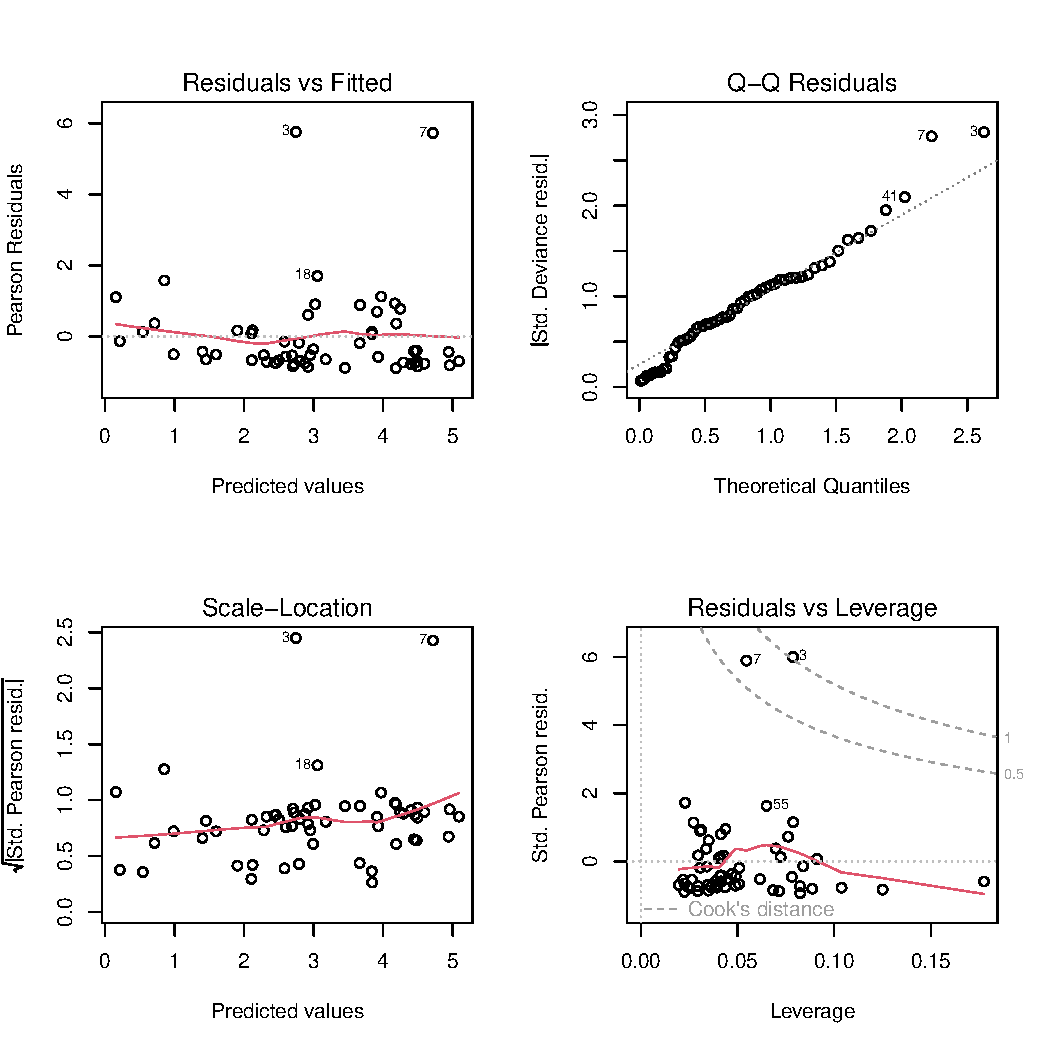
\includegraphics[width=\textwidth]{HelmBiogeog/Figures/HostDiv_diagnostics.pdf}
    \caption[Host richness model diagnostics]{Model diagnostics plots for our negative binomial model of \textbf{host richness} across islands, including residual vs fitted values (top left), Q-Q plot (top right), scale-location (bottom left), and residual vs leverage plot (bottom right), with dotted lines representing Cook's distance contours of 0.5 and 1, respectively. }
    \label{fig:hostDivdiagnostics}
  \end{center}
\end{figure}

\begin{figure}[H]
  \begin{center}
    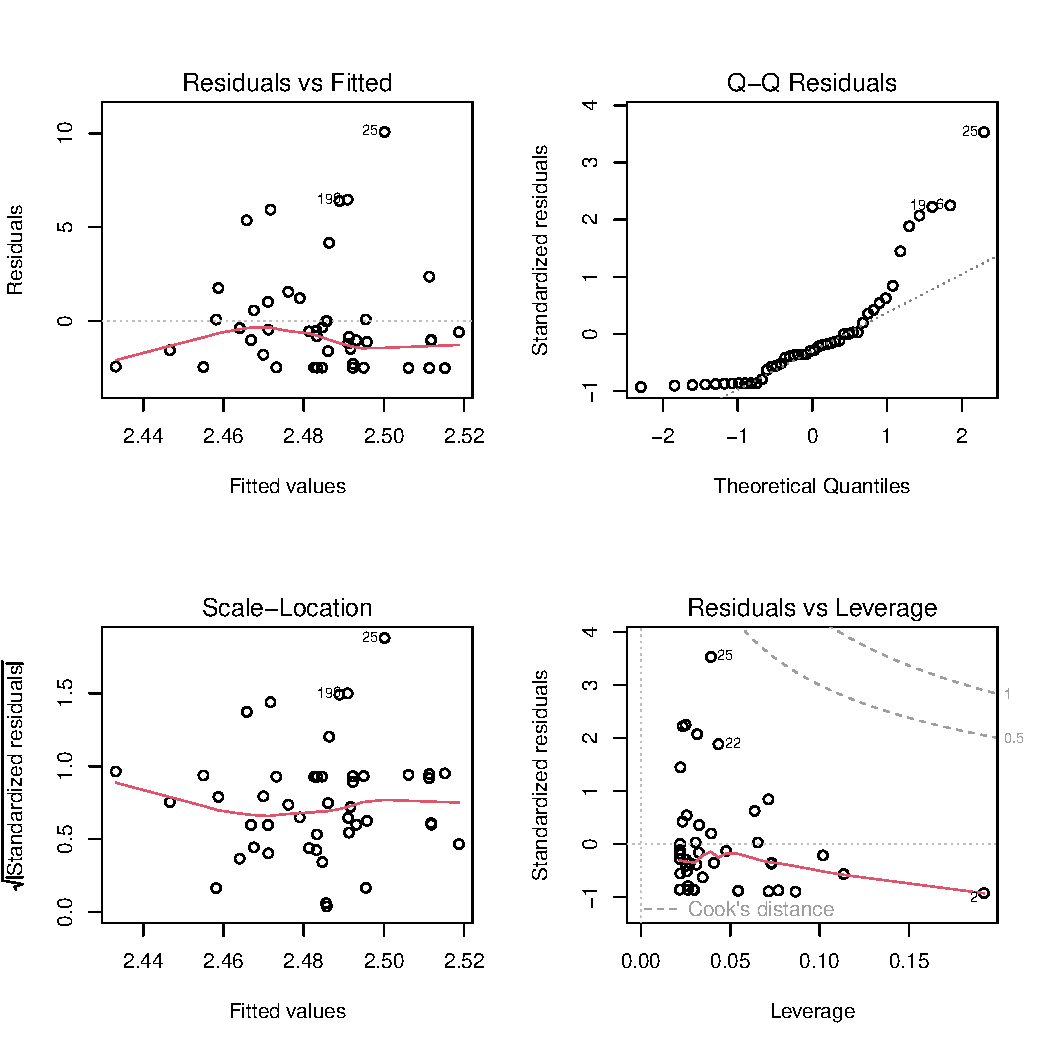
\includegraphics[width=\textwidth]{HelmBiogeog/Figures/NODFc_Distance_diagnostics.pdf}
    \caption[$NODF_c$ model diagnostics]{Model diagnostics plots for our generalized linear model of \textbf{network nestedness ($NODF_c$)} across islands, including residual vs fitted values (top left), Q-Q plot (top right), scale-location (bottom left), and residual vs leverage plot (bottom right), with dotted lines representing Cook's distance contours of 0.5 and 1, respectively. }
    \label{fig:nodfcdiagnostics}
  \end{center}
\end{figure}